\newlength\mystoreparindent
\newenvironment{myparindent}[1]{%
\setlength{\mystoreparindent}{\the\parindent}
\setlength{\parindent}{#1}
}{%
\setlength{\parindent}{\mystoreparindent}
}

\documentclass[a4paper]{article}
\usepackage{amssymb}
\usepackage{amsthm}
\usepackage{mathtools}
\usepackage{enumitem}
\usepackage{graphicx}

\DeclarePairedDelimiterX{\infdivx}[2]{(}{)}{%
  #1\;\delimsize\|\;#2%
}
\newcommand{\infdiv}{D\infdivx}
\DeclarePairedDelimiter{\norm}{\lVert}{\rVert}

\newtheorem{theorem}{Theorem}[section]
\newtheorem{corollary}{Corollary}[theorem]
\newtheorem{lemma}[theorem]{Lemma}

\graphicspath{ {./} }

\begin{document}

\begin{myparindent}{0pt}

Kyle Kloberdanz \newline
21 February 2022 \newline

\textbf{Exercise 2.3.3}:
Let $f = x^5 + 2x^4 + 2x^3 - x^2 - 2x - 2$ and $g = 4x^4 + 16$. Find $gcd(f, g)$
and express it as $uf + vg$
\newline

I spent too much time trying to show long division in LaTex. I gave up, and
inserted a scanned image of my notes instead to show the process of calculating
the GCD using the Euclidean Algorithm below. From those results, we can see that
the monic form of the $GCD(f, g) = x^2 + 2x + 2$.

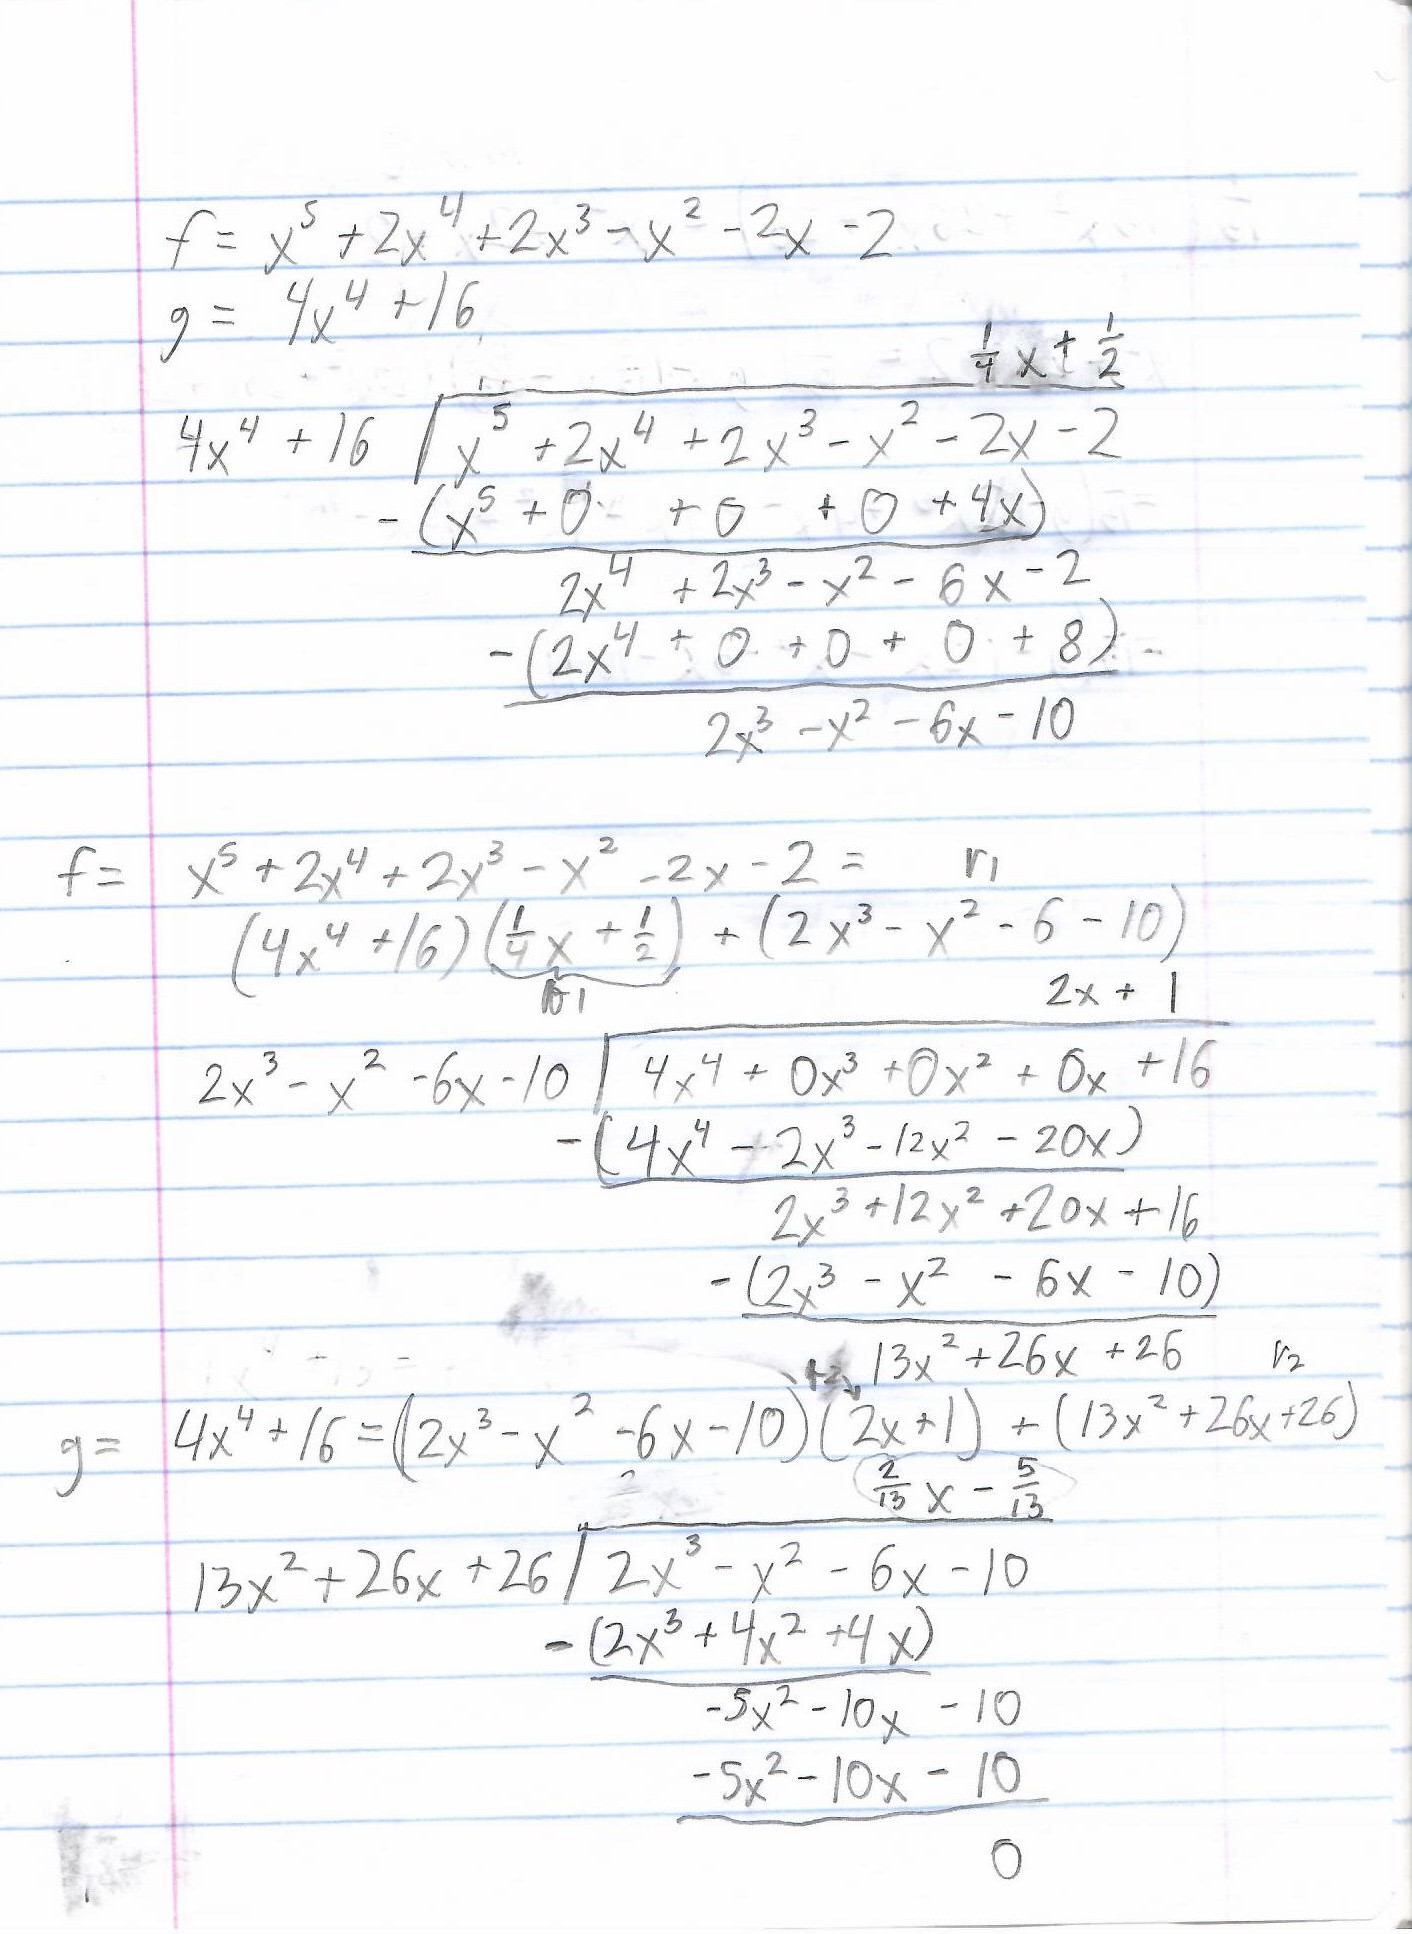
\includegraphics{longdivision}

\textbf{Exercise 2.3.5}:
Prove that a polynomial $f \in \mathbb{F}[x]$ of degree 3 is irreducible in
$\mathbb{F}[x]$ if it does not have a root in $\mathbb{F}$.
\newline
\begin{proof}
  Recall, for a polynomial $f$ to be irreducible, one must be able to write
  $f = uv$ where either $u$ or $v$ is a nonzero constant polynomial, i.e.,
  either $deg(u) = 0$ or $deg(v) = 0$. \newline

  We will demonstrate a proof by contrapositive where we will show that a
  polynomial $f \in \mathbb{F}[x]$ of degree 3 has
  a root in $\mathbb{F}$ if $f$ is not irreducible (i.e., $f$ is reducible) in
  $\mathbb{F}[x]$
  \newline

  Because we are assuming that $f$ is reducible, then we can write $f = uv$
  where $deg(u) > 0$ and $deg(v) > 0$. Because $deg(uv) = deg(u) + deg(v)$ and
  $deg(f) = 3$ (as per the problem statement), then we have two cases, either
  $deg(u) = 1$ and $deg(v) = 2$ or $deg(u) = 2$ and $deg(v) = 1$. \newline

  Let's start by assuming that $deg(u) = 1$. This means that $u = a_0 + a_1x$
  where $a_0, a_1 \in \mathbb{F}$. Because $\mathbb{F}$ is a field, and
  $a_1 \neq 0$ (because if $a_1 = 0$ then $deg(u) = 0$, which would be a
  contradiction to the statement that $deg(u) = 1$)
  then there
  exists a multiplicative inverse for $a_1$ in $\mathbb{F}$, namely
  $a_1^{-1}$, such that $u(-a_0a_1^{-1}) = a_0 + a_1(-a_0a_1^{-1}) = a_0 + (-a_0) = 0$
  therefore $f$ has the root $-a_0a_1^{-1} \in \mathbb{F}$. \newline

  Since we have shown that a polynomial $f \in \mathbb{F}[x]$ of degree 3 has a
  root in $\mathbb{F}$ if $f$ is reducible in $\mathbb{F}[x]$, by the
  contrapositive we see that a polynomial $f \in \mathbb{F}[x]$ of degree 3 is
  irreducible in $\mathbb{F}[x]$ if it does not have a root in $\mathbb{F}$.
\end{proof}

\textbf{Exercise}:
Come up with a polynomial $g \in \mathbb{Q}[x]$ that has no roots in $\mathbb{Q}$
but is \textit{not} irreducible. \newline

let $g = x^4 + 2x^2 + 1 = (x^2 + 1)(x^2 + 1)$ \newline

We can see that $g$ is not irreducible. \newline

To avoid having to apply the quartic equation, by factoring this polynomial, we
see that all of the roots will be $x$ such that $x^2 + 1 = 0$. Hence we can
apply the quadratic equation to find the roots like so.

\[
  \frac{-0 \pm \sqrt{0^2 - 4(1)(1)}}{2(1)} = \frac{\pm \sqrt(-4)}{2} =
  \frac{\pm 2 \sqrt{-1}}{2} = \pm \sqrt{-1} = \pm i \notin \mathbb{Q}
\]

Hence, we see that the roots to $g = x^4 + 2x^2 + 1$ are $i$ and $-i$, which
do not exist in $Q$, and is therefore an example of a polynomial
$g \in \mathbb{Q}[x]$ that has no roots in $\mathbb{Q}$ but is not irreducible.
\newline

\textbf{Exercise 2.3.6}:
Consider the polynomial $f(x) = x^3 - x + 2 \in \mathbb{Z}_5[x]$ (more precisely,
$f(x) = [1]x^3 - [1]x + [2]$). Prove that $f$ is irreducible in $\mathbb{Z}_5$.
\textit{Hint: Use Exercise 2.3.5}.
\newline
\begin{proof}
  Recall that we have proven in Exercise 2.3.5 that if a polynomial
  $f \in \mathbb{F}[x]$ of degree 3 does not have a root in $\mathbb{F}$, then
  $f$ is irreducible if $\mathbb{F}[x]$. \newline

  We will therefore show that $f \in \mathbb{Z}_5[x]$ does not have a root in
  $\mathbb{Z}_5$, and is therefore irreducible. \newline

  Because $\mathbb{Z}_5$ is the finite set $\{0, 1, 2, 3, 4\}$, we can show
  that given any $x \in \mathbb{Z}_5$, $x^3 - x + 2 \neq 0$ as follows.
  \newline

  $f(0) = 2 \neq 0$ \newline
  $f(1) = 1 - 1 + 2 = 2 \neq 0$ \newline
  $f(2) = 2^3 - 2 + 2 = 8 - 2 + 2 \equiv 8 \pmod{5} = 3 \neq 0$ \newline
  $f(3) = 3^3 - 3 + 2 = 8 - 2 + 2 = 27 - 3 + 2 \equiv 26 \pmod{5} = 1 \neq 0$ \newline
  $f(4) = 4^3 - 4 + 2 = 64 - 4 + 2 \equiv 62 \pmod{5} = 2 \neq 0$ \newline

  We have exhausted every possible value for $x \in \mathbb{Z}_5$, and found
  that no such value for $x$ is a root for $f$, i.e., where $f(x) = 0$, hence
  there does not exist a root for $f$ in $\mathbb{Z}_5$, therefore by Exercise
  2.3.5, we conclude that $f$ is irreducible in $\mathbb{Z}_5$.
\end{proof}

\textbf{Exercise}:
Consider the polynomial $p(x) = 3x^3 + 2x^2 + 4x + 2 \in \mathbb{Z}_7[x]$
(more precisely, $f(x) = [3]x^3 + [2]x^2 + [4]x + [2]$). Prove that $f$ is
\textit{not} irreducible in $\mathbb{Z}_7[x]$.


\begin{proof}
  Recall that we have proven in Exercise 2.3.5 that if a polynomial
  $f \in \mathbb{F}[x]$ of degree 3 does not have a root in $\mathbb{F}$, then
  $f$ is irreducible if $\mathbb{F}[x]$. \newline

  This means that if a polynomial
  $f \in \mathbb{F}[x]$ of degree 3 does have a root in $\mathbb{F}$, then
  $f$ is not irreducible if $\mathbb{F}[x]$. \newline

  We will show that $f$ has a root in $\mathbb{F}$. \newline

  $f(0) = 2 \neq 0$ \newline
  $f(1) = 3 + 2 + 4 + 2 \equiv 11 \pmod 7 = 2 \neq 0$ \newline
  $f(2) = 24 + 8 + 8 + 2 \equiv 42 \pmod 7 = 0$ \newline

  We have found a root $2 \in \mathbb{Z}_7$ for $f \in \mathbb{Z}_7[x]$.
  Therefore, because the polynomial $f \in \mathbb{Z}_7[x]$ of degree 3 has a
  root in $\mathbb{Z}_7$, $f$ is not irreducible.
\end{proof}

As a bonus, by using the Computer Algebra System, sage mathematics,
one can find that factors for this polynomial are $(3x + 1)(x^2 + 5x + 2)$,
therefore $p(x)$ is not irreducible.

\begin{verbatim}
sage: x = PolynomialRing(RationalField(), 'x').gen()
sage: f = (3*x^3 + 2*x^2 + 4*x + 2)
sage: f.factor_mod(7)
(3) * (x + 5) * (x^2 + 5*x + 2)
\end{verbatim}

\textbf{Exercise 2.5.1}:
Suppose $T:R^n \rightarrow R^n$ is a linear transformation. Prove that $T$ is
an isometry if and only if $T(v) \cdot T(w) = v \cdot w$. Recall that an
isometry is a \textit{bijection} that preserves distance.

\textit{Note}: when
proving that if $T(v) \cdot T{w} = v \cdot w$ then $T$ is an isometry,
make sure you verify that $T$ is a bijection.
\newline
\begin{proof}
\end{proof}

\end{myparindent}
\end{document}
